\documentclass[nofonts]{tufte-handout}

\usepackage{polyglossia}
\setdefaultlanguage{french}
\usepackage{booktabs}
\usepackage[locale=FR]{siunitx}
\usepackage{graphicx}
\usepackage{enumitem}
\usepackage{tikz}
\usepackage{amsmath}

\usepackage{fontspec}
\usepackage{ifluatex}
\setmainfont[Renderer=Basic, Numbers=OldStyle, Scale = 1.0]{TeX Gyre Pagella}
\setsansfont[Renderer=Basic, Scale=0.90]{TeX Gyre Heros}
\setmonofont[Renderer=Basic]{TeX Gyre Cursor}
\ifluatex
  \newcommand{\textls}[2][5]{%
    \begingroup\addfontfeatures{LetterSpace=#1}#2\endgroup
  }
  \renewcommand{\allcapsspacing}[1]{\textls[15]{#1}}
  \renewcommand{\smallcapsspacing}[1]{\textls[10]{#1}}
  \renewcommand{\allcaps}[1]{\textls[15]{\MakeTextUppercase{#1}}}
  \renewcommand{\smallcaps}[1]{\smallcapsspacing{\scshape\MakeTextLowercase{#1}}}
  \renewcommand{\textsc}[1]{\smallcapsspacing{\textsmallcaps{#1}}}
\fi

\sisetup{
  mode=text,
  reset-text-family=false,
  reset-text-series=false,
  per-mode=symbol,
}

\newcommand{\F}{\boldsymbol{\vec{F}}}
\newcommand{\vv}{\boldsymbol{\vec{v}}}
\newcommand{\va}{\boldsymbol{\vec{a}}}

\newif\ifsolution
%\solutiontrue  % Montrer les solutions dans le pdf
\solutionfalse  % Cacher les solutions


\title{Exercices de révision de mécanique}
\author{Loïc Séguin-Charbonneau}
\date{203-NYB-05, Automne 2024}

\begin{document}

\maketitle

\section{Lancer du marteau}

\begin{marginfigure}[10\baselineskip]
  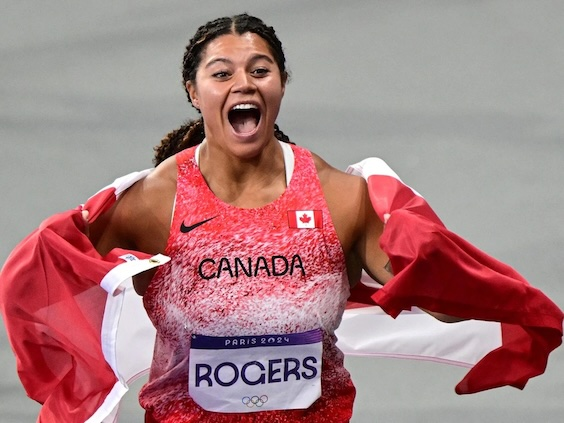
\includegraphics[width=\marginparwidth]{figures/camryn_rogers.jpg}
  \caption{Camryn Rogers après avoir gagné la médaille d'or aux Jeux olympiques
  de Paris. Photo par Martin Bernetti/AFP (\citet{hill_2024})}
\end{marginfigure}
Aux Jeux olympiques de Paris, la Canadienne Camryn Rogers a lancé le marteau à
une distance de \qty{76.97}{\meter} ce qui lui a valu la médaille d'or. Vous
pouvez voir le lancer sur la chaîne Youtube de CBC Sports\cite{youtube_cbc}. L'angle
que faisait la vitesse du marteau avec l'horizontal au moment du lancer était
de \qty{39.02}{\degree}. À ce moment, le boulet était environ à la
hauteur de la tête de l'athlète, soit \qty{170}{\centi\meter}. La longueur du marteau est
de \qty{1195}{\milli\meter} et sa masse de \qty{4}{\kilo\gram}.

\begin{enumerate}[label=\alph*)]
  \item Quelle était la vitesse du marteau au moment de le lâcher?
  \item Quelle était la hauteur maximale atteinte par le marteau?
  \item Juste avant de lâcher le marteau, quelle force devait exercer Camryn
    pour le maintenir en rotation?
\end{enumerate}


\ifsolution
\subsection{Solution}

\begin{marginfigure}[4\baselineskip]
  \begin{tikzpicture}[>=stealth]
    \draw[<->] (0, 2) node[left] {$y$} -- (0, 0) -- (4, 0) node[below] {$x$};
    \fill (0, 1) circle (2pt);
    \draw[densely dashed, domain=0:3.3] plot (\x, 1 + \x - 0.4 * \x * \x);
    \draw[thick, ->] (0, 1) -- ++(42:1) node[above] {$\vv_0$};
    \draw[thick, ->] (0, 1) -- ++(0, -0.6) node[left] {$\va$};
    \draw (0, 1) -- ++(-0.15, 0) node[left] {$y_0$};
    \draw (3.27, 0) -- ++(0, -0.15) node[below] {$D$};
    \draw (0, 1) -- (0.4, 1) arc (0:42:0.4);
    \node at (0.6, 1.2) {$\theta$};
  \end{tikzpicture}
\end{marginfigure}
\begin{enumerate}[label=\alph*)]
  \item Quand Camryn lâche le marteau, il se déplace uniquement sous l'influence
    de la gravité (en négligeant la résistance de l'air) donc il décrit un
    mouvement de projectile. Avec le système d'axe ci-contre, on sait que les
    composantes de la position seront données par les deux équations
    \begin{align}
      x &= x_0 + v_{0x} t + \frac{1}{2} a_x t^2  \label{eq:marteau_x_gen}\\
      y &= y_0 + v_{0y} t + \frac{1}{2} a_y t^2  \label{eq:marteau_y_gen}
    \end{align}
    L'accélération pointe vers les $y$ négatifs, donc $a_x = 0$ et $a_y = -g =
    -\qty{9.81}{m/s^2}$. La composante
    $x$ de la position initiale est nulle en raison du choix d'origine du
    d'axe. Les composantes de la vitesse initiale peuvent être trouvées avec un
    peu de trigonométrie. La composante $y$ de la position initiale est $y_0 =
    \qty{170}{cm}$. En substituant dans les équations générales
    \ref{eq:marteau_x_gen} et \ref{eq:marteau_y_gen} on obtient les équations
    adaptées au problème
    \begin{align}
      x &= v_{0}\cos(\theta) t  \label{eq:marteau_x_adapte}\\
      y &= y_0 + v_{0}\sin(\theta) t - \frac{1}{2} g t^2  \label{eq:marteau_y_adapte}
    \end{align}
    On peut isoler $t$ dans l'équation \ref{eq:marteau_x_adapte}
    \begin{equation}
      t = \frac{x}{v_0 \cos(\theta)}
    \end{equation}
    puis remplacer dans l'équation \ref{eq:marteau_y_adapte} 
    \begin{align}
      y &= y_0 + v_{0}\sin(\theta) \frac{x}{v_0 \cos(\theta)} - \frac{1}{2} g
           \left( \frac{x}{v_0 \cos(\theta)} \right) ^2  \\
        &= y_0 + x \tan(\theta)  - \frac{1}{2} g
           \left( \frac{x}{v_0 \cos(\theta)} \right) ^2
    \end{align}
    On peut maintenant utiliser le point de la trajectoire où le marteau touche
    le sol: $x = D = \qty{76.97}{m}$ et $y = 0$ pour obtenir
    \begin{align}
      0 &= y_0 + D \tan(\theta)  - \frac{1}{2} g
           \left( \frac{D}{v_0 \cos(\theta)} \right) ^2  \\
      v_0 &= \frac{D}{\cos(\theta)} \sqrt{
        \frac{g/2}{y_0 + D\tan(\theta)}
      }  \\
        &= \qty{27.41}{m/s}  \nonumber
    \end{align}
    La vitesse initiale du marteau est donc de \qty{27.41}{m/s} à
    \qty{39.02}{\degree} au-dessus de l'horizontale.

  \item Au sommet de la trajectoire, la composante verticale de la vitesse est
    nulle. L'équation générale de la vitesse en fonction du temps est
    \begin{equation}
      v_y = v_{0y} + a_y t
    \end{equation}
    et l'équation adaptée est au sommet de la trajectoire est donc
    \begin{equation}
      0 = v_{0}\sin\theta - g t
    \end{equation}
    On peut isoler le temps
    \begin{equation}
      t = \frac{v_{0}\sin\theta}{g}
    \end{equation}
    et remplacer dans l'équation pour la composante $y$ de la vitesse en
    fonction du temps (équation \ref{eq:marteau_y_adapte})
    \begin{align}
      y &= y_0 + v_{0}\sin(\theta) \frac{v_{0}\sin\theta}{g} - \frac{1}{2} g
      \left(\frac{v_{0}\sin\theta}{g}\right)^2  \\
        &= y_0 + \frac{1}{2} \frac{v_{0}^2\sin^2\theta}{g}  \\
        &= \qty{16.88}{m}  \nonumber
    \end{align}

  \item Lorsque Camryn tient le marteau, celui-ci effectue un mouvement
    circulaire. La force exercée par Camryn est dans la direction radiale et on
    peut négliger l'apporte de la force de gravité (pouquoi?). La force exercée
    par Camryn est donc la force centripète. L'accélération centripète d'un
    objet en mouvement circulaire de rayon $r$ à une vitesse de grandeur $v$ est
    \begin{align}
      a_r = \frac{v^2}{r}
    \end{align}
    En combinant avec la deuxième loi de Newton, on a donc que la force est
    \begin{align}
      F = ma_r = \frac{mv^2}{r}
    \end{align}
    La masse est celle du marteau, la vitesse juste avant le lancer est la
    vitesse initiale trouvée en a). Le rayon de la trajectoire est la somme de
    la longueur du marteau et la longueur des bras de Camryn (approximativement
    \qty{60}{cm}). En substituant ces valeurs, on trouve que Camryn doit exercer
    une force de \qty{1674}{N} vers elle.
\end{enumerate}
\fi


\section{Énergie et puissance d'un barrage hydroélectrique}

La centrale hydroélectrique Robert-Bourassa sur la rivière La Grande est une
centrale à réservoir. L'eau du réservoir chute d'une hauteur de
\qty{137.16}{\meter} (voir \cite{hydroquebec_centrales}) et fait tourner une turbine
reliée à une génératrice. La centrale produit une puissance électrique maximale
de \qty{5616}{\mega\watt}.

\begin{enumerate}[label=\alph*)]
  \item Quelle est l'énergie potentielle d'un kilogramme d'eau au sommet du réservoir?
  \item Quelle est l'énergie cinétique d'un kilogramme d'eau juste avant qu'il
    ne touche la turbine en bas du réservoir?
  \item La centrale a une efficacité de \qty{90}{\percent}, c'est-à-dire que
    \qty{90}{\percent} de l'énergie cinétique de l'eau qui tombe peut être
    convertie en énergie électrique. Quelle quantité d'énergie électrique est
    produit par la chute d'un kilogramme d'eau?
  \item Quelle masse d'eau est requise pour produire \qty{5616}{\mega\joule} d'énergie?
  \item Quel débit d'eau (c'est-à-dire le volume par unité de temps) doit
    tomber pour produire une puissance de \qty{5616}{\mega\watt}? (Vous pouvez
    vérifier l'ordre de grandeur de votre réponse en utilisant l'outil des
    débits d'Hydro Québec \cite{hydroquebec_debit}.)
\end{enumerate}

\ifsolution
\subsection{Solution}
\begin{enumerate}[label=\alph*)]
  \item L'énergie potentielle gravitationnelle est $U_g = mgh$, donc pour une
    masse d'un kilogramme à une hauteur de \qty{137.16}{m}, on obtient $U_g =
    \qty{1345.5}{J}$.
  \item Si on néglige tous les frottements, la seule force à considérer est la
    force gravitationnelle qui est une force conservative. Par conséquent le
    principe de conservation de l'énergie s'applique et la variation d'énergie
    cinétique est l'opposée de la variation d'énergie potentielle. En supposant
    que l'énergie cinétique de l'eau au sommet du réservoir est nulle, on a donc
    que l'énergie cinétique d'un kilogramme d'eau en bas du réservoir est de
    \qty{1345.5}{J}.
  \item On multiplie simplement l'énergie cinétique par 90\% ce qui donne
    \qty{1211}{J}.
  \item Il suffit de diviser l'énergie totale par l'énergie produite par un
    kilogramme pour savoir combien de kilogrammes sont requis. On trouve
    \qty{4.638e6}{kg} soit \qty{4638}{tonnes}.
  \item On sait que \qty{1}{L} d'eau a une masse de \qty{1}{kg}. La masse
    trouvée en d) est donc équivalente à \qty{4.638e6}{L}. Une puissance de
    \qty{5616}{MW} correspond à une production d'énergie de \qty{5616}{MJ} à
    chaque seconde. Le débit d'eau qui doit tomber est donc de \qty{4.638}{ML/s}.
\end{enumerate}
\fi


\section{Forces sur un vaisseau spatial}

Un satellite de \qty{156}{\kilogram} est en orbite autour de la Terre à une
altitude de \qty{400}{\kilo\meter}. Le satellite allume un propulseur qui
éjecte un gaz générant une force $\F_p$ de \qty{170}{\newton} qui
fait un angle de \SI{125}{\degree} avec la vitesse du vaisseau (voir la figure
ci-contre).
\begin{marginfigure}[-4\baselineskip]
  \begin{tikzpicture}[>=stealth, scale=0.8]
    \clip (-2, -0.5) rectangle (2, 3.8);
    \draw (0, 0) circle (2cm);
    \fill[black!70] (0, 0) circle (12px);
    \begin{scope}[shift={(0.3, 2.2cm)}, scale=0.3, rotate=150]
      \draw[fill=black!60] (0, 0) rectangle (1, 2);
      \draw (0.5, 2) -- ++(80:0.9);
      \draw (0.5, 2) -- ++(100:1.1);
      \draw (1, 1) -- ++(10:1) rectangle ++(0.4, 0.6);
      \draw (0, 1) -- ++(190:1) rectangle ++(-0.4, +0.6);
    \end{scope}
    \draw[ultra thick, ->] (0, 2) -- ++(1, 0) node[above] {$\vv$};
    \draw[ultra thick, ->] (0, 2) -- ++(125: 1.3) node[above] {$\F_p$};
    \draw (0.5, 2) arc (0: 125: 0.5);
    \node at (0.4, 2.6) {\qty{125}{\degree}};
  \end{tikzpicture}
\end{marginfigure}

Quelle est la force nette qui agit sur le satellite?


\section{Un vol d'une seconde}
\marginnote{Chapitre 1, exercice 1.10.5 dans \citet{seguin_mec_2024}}
À quel angle doit-on lancer une balle à \qty{8}{\meter\per\second} pour qu'elle
reste dans les airs pendant \qty{1}{\second}?


\section{Volleyball}
\marginnote{Chapitre 4, P27 dans \citet{lafrance_mec_2014}}
Au volleyball, le filet a une hauteur de \qty{2.43}{\meter} et il est situé à
une distance de \qty{9}{\meter} du serveur. Ce dernier frappe le ballon à une
vitesse de \qty{12.4}{\meter\per\second}, formant un angle de
\qty{24.0}{\degree} au-dessus de l'horizontale et à une hauteur de
\qty{2.2}{\meter}.
\begin{enumerate}[label=\alph*)]
  \item À quelle hauteur au-dessus du filet le ballon passe-t-il?
  \item Donnez le module et l'orientation de la vitesse à ce moment.
  \item À quelle distance du filet le ballon frappe-t-il le sol?
\end{enumerate}


\section{Plan incliné}
\marginnote{Chapitre 6, E21 dans \citet{benson_mec_2024}}
Deux blocs de masses égales $m_1 = m_2 = \qty{5}{\kilo\gram}$ sont reliés entre
eux et suspendus à une poulie. On donne $\mu_c = \num{0.25}$ pour le bloc 2.
Trouver le module de l'accélération des deux blocs sachant que $m_1$ se déplace
vers le bas.
\begin{marginfigure}
  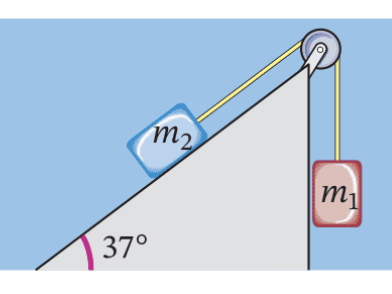
\includegraphics[width=\marginparwidth]{figures/benson_c6e21.png}
\end{marginfigure}


\section{Réponses}

\noindent Lancer du marteau: a) \qty{27.41}{m/s} à \qty{39.02}{\degree}
au-dessus de l'horizontale; b) \qty{16.88}{m}; c) \qty{1674}{N}

\noindent Centrale hydroélectrique: a) \qty{1345.5}{J}
    b) \qty{1345.5}{J}
    c) \qty{1211}{J}
    d) \qty{4.638e6}{kg}
    e) \qty{4.638}{ML/s}

\noindent Vaisseau spatial: \qty{1221}{N} à \qty{94.58}{\degree} horaire par
rapport à la vitesse initiale

\noindent Un vol d'une seconde : \qty{37.8}{\degree} au-dessus de l'horizontal

\noindent Volleyball: a) \qty{0.68}{\meter};
            b) \qty{11.7}{\meter\per\second} à \qty{13.6}{\degree} sous l'horizontale;
            c) \qty{6.4}{\meter}

\noindent Plan incliné: \qty{0.980}{\meter\per\second\squared}

\bibliography{../elecmag}
\bibliographystyle{plainnat}

\end{document}

